\begin{figure}[H]
\begin{changemargin}{0cm}{0cm}
  \begin{center}
    \begin{minipage}[h]{0.6\linewidth}
        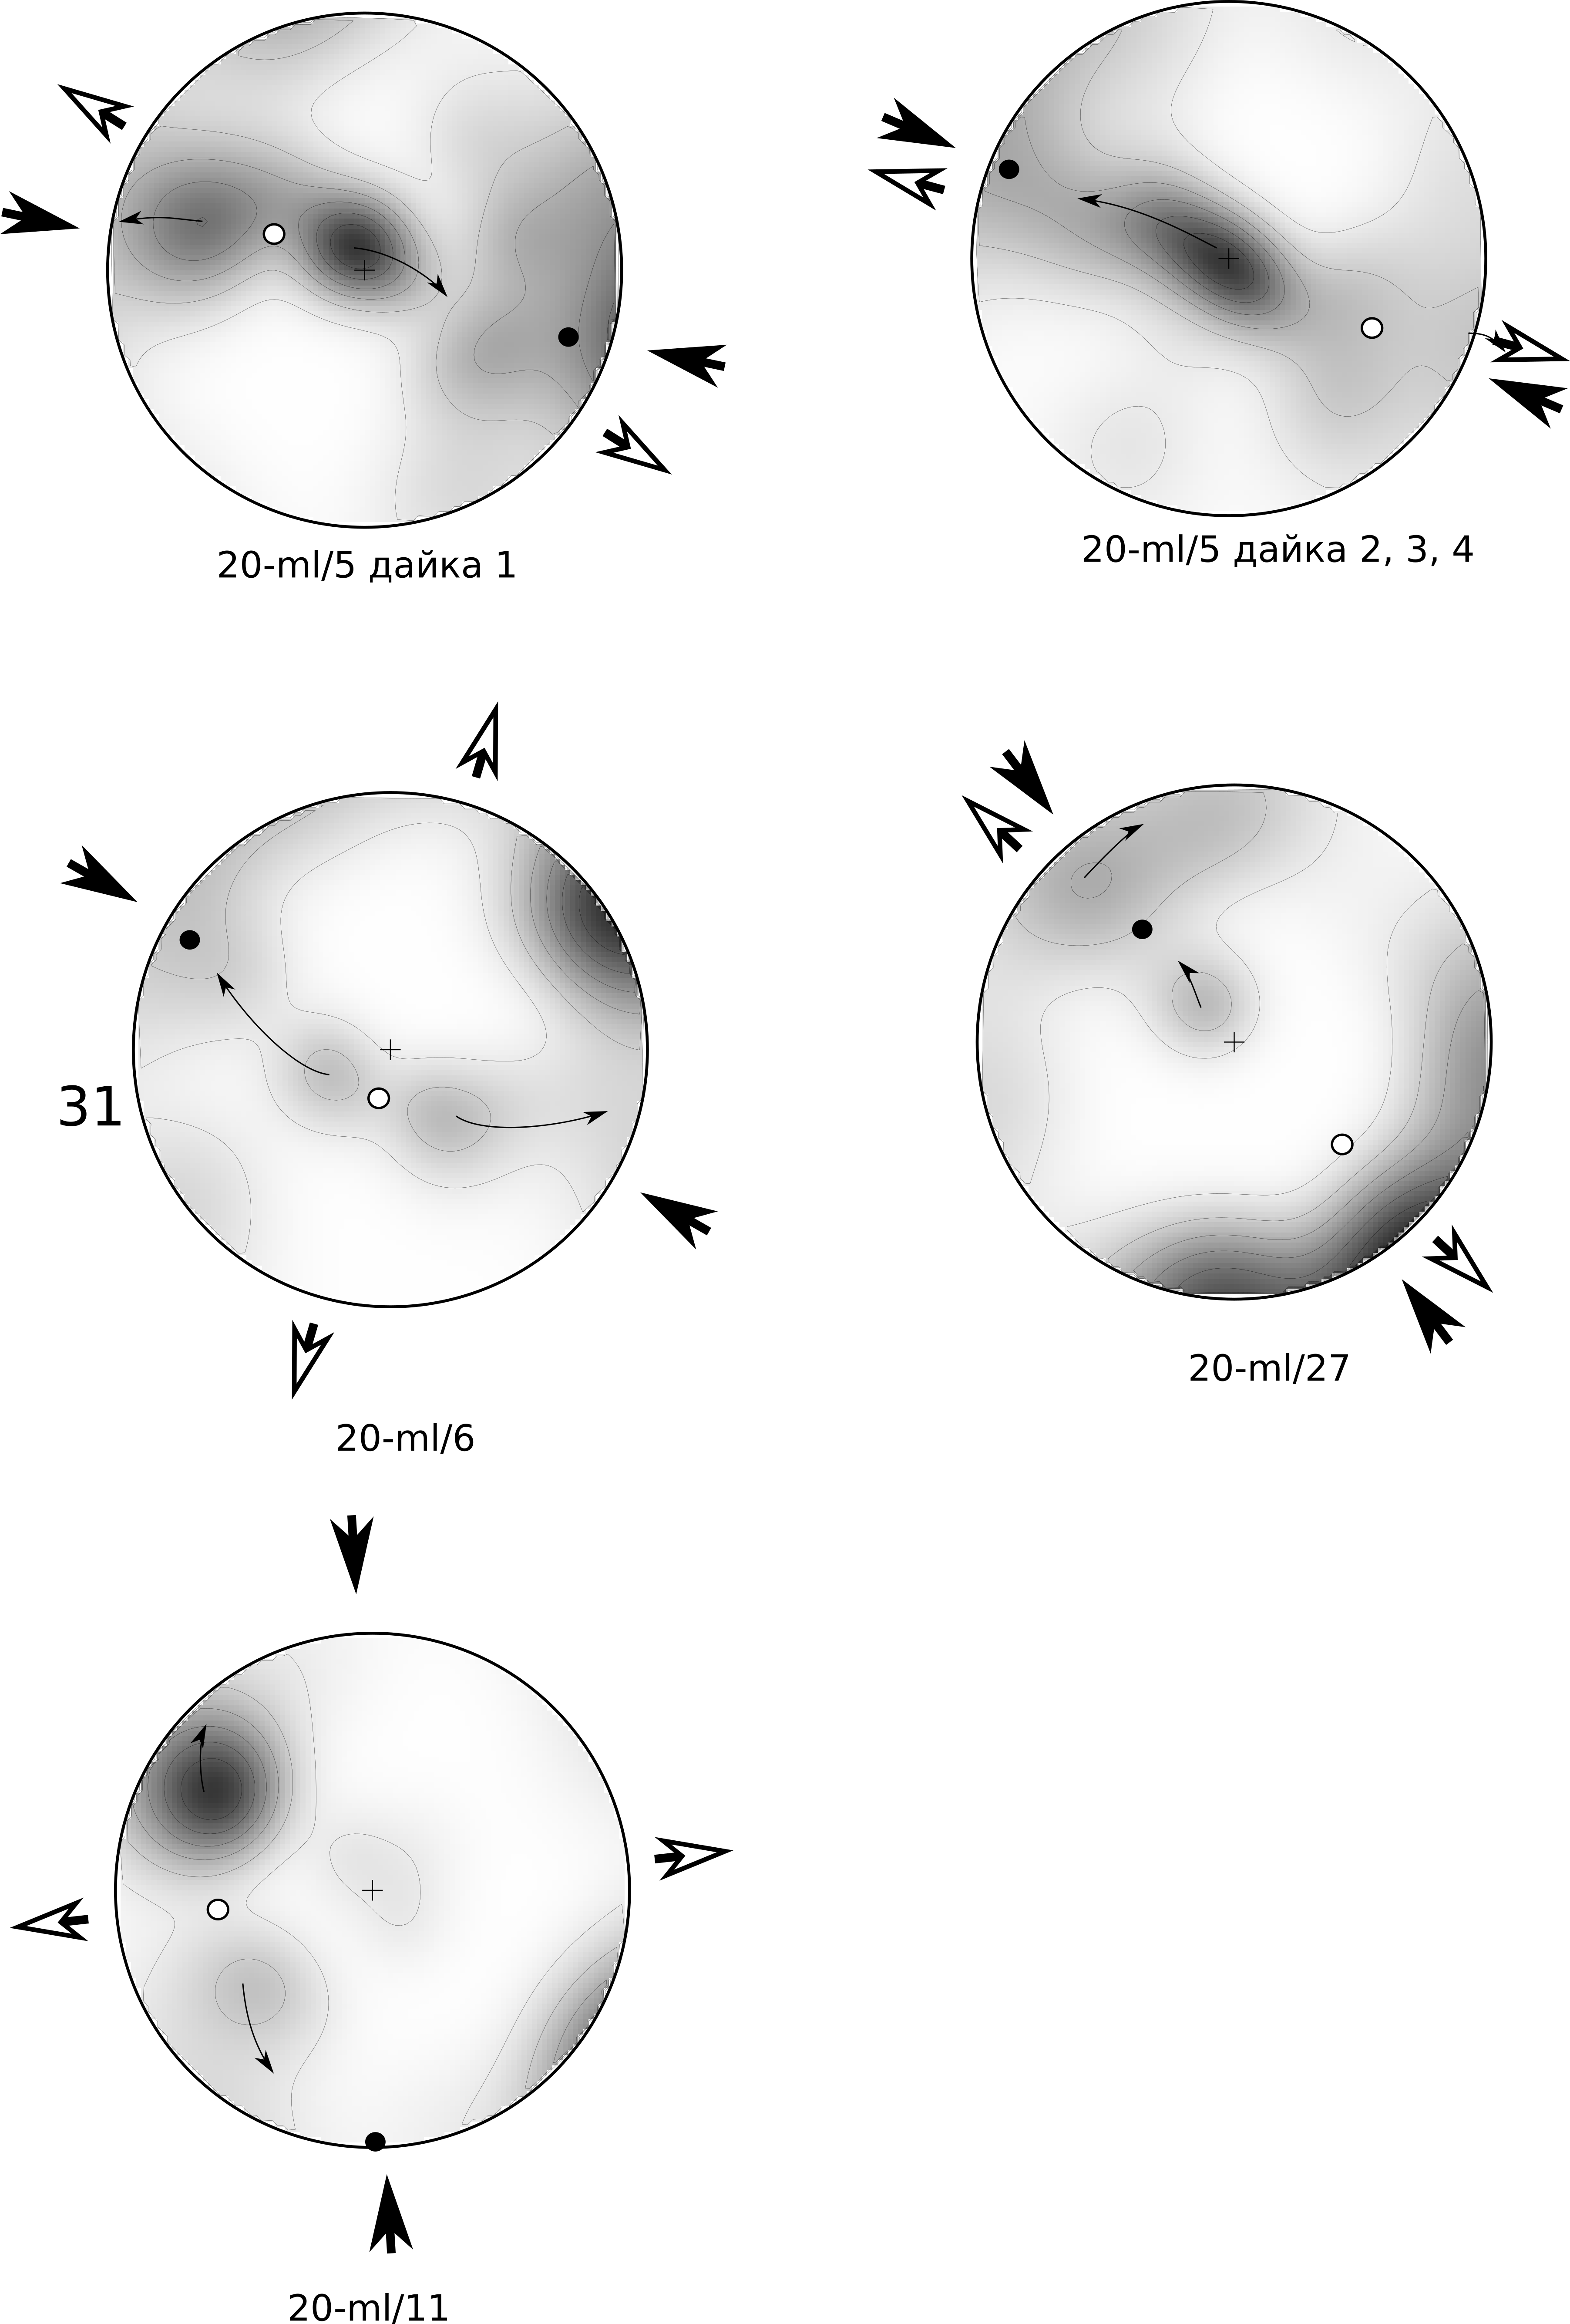
\includegraphics[width=1\textwidth]{authors/kondratev-fig2.png}
        \caption{Матрицы плотности тектонической трещиноватости и ориентация осей сжатия и растяжения восстановленные методом Николаева}
        \label{fig:kondratev-fig2}
    \end{minipage}
\hfill
    \begin{minipage}[h]{0.33\linewidth}
      \begin{center}
              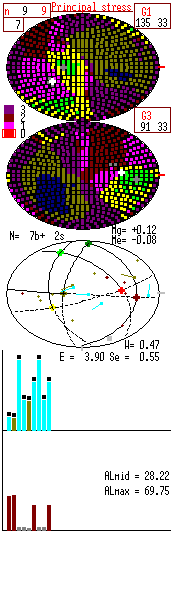
\includegraphics[width=0.75\textwidth]{authors/kondratev-fig3.png}
      \end{center}

        \caption{Стереограмма напряженного состояния на основе
    анализа массива зеркал скольжения методом катакластического анализа разрывных смещений Ю.\,Л.\,Ребецкого.
    Нижняя полусфера. Желтым цветом выделен выход на полусферу оси $\upsigma_1$, красным цветом~--- $\upsigma_3$.}
        \label{fig:kondratev-fig3}
    \end{minipage}


  \end{center}
\end{changemargin}

\end{figure}
